\section{Mitochondrial DNA and human evolution A review (Ева)}

\subsection{Нормальное название}

Митохондриальная ДНК и эволюция человека.

\subsection{Абстракт}

\begin{enumerate}
	\item Часть клеточной ДНК содержится в митохондрия 
	
	\item Изучение этой ДНК позволяет определить происхождение нашего вида, родство, возможное скрещивание с другими гоминидами (семейство приматов, включающих людей и больших человекообразных обезьян), миграции и колонизацию новых регионов мира с материнской точки зрения
\end{enumerate}

\subsubsection{Общая инфа}

1)	Копий такой молекулы в клетке от 100 до 1000 (вероятность обнаружения в образцах выше и больше материала)

2)	В молекуле явно отсутствует рекомбинация, что означает, что все различия между последовательностями мтДНК являются результатом только фиксированных изменений. Было доказано, что частота мутаций в митохондриальных геномах в несколько раз выше, чем в ядерных последовательностях. Таким образом, это вызывает высокий уровень вариабельности последовательностей между людьми, накопленный за относительно короткий период времени по отношению к общей предковой молекуле мтДНК.

3)	Постоянная скорость эволюционных изменений может служить молекулярными часами, позволяя исследовать возраст определенных линий и время их разрыва.

Ключевые понятия:

\textbf{Гаплогруппа} — группа схожих гаплотипов, имеющих общего предка, у которого произошла мутация, унаследованная всеми потомками.

\textbf{Гаплотип} — совокупность аллелей на локусах одной хромосомы, обычно наследуемых вместе.

\textbf{Аллели} — различные формы одного и того же гена, расположенные в одинаковых участках гомологичных хромосом, определяют направление развития конкретного признака

\subsection{Картинки}

\begin{figure}[H]
	\centering
	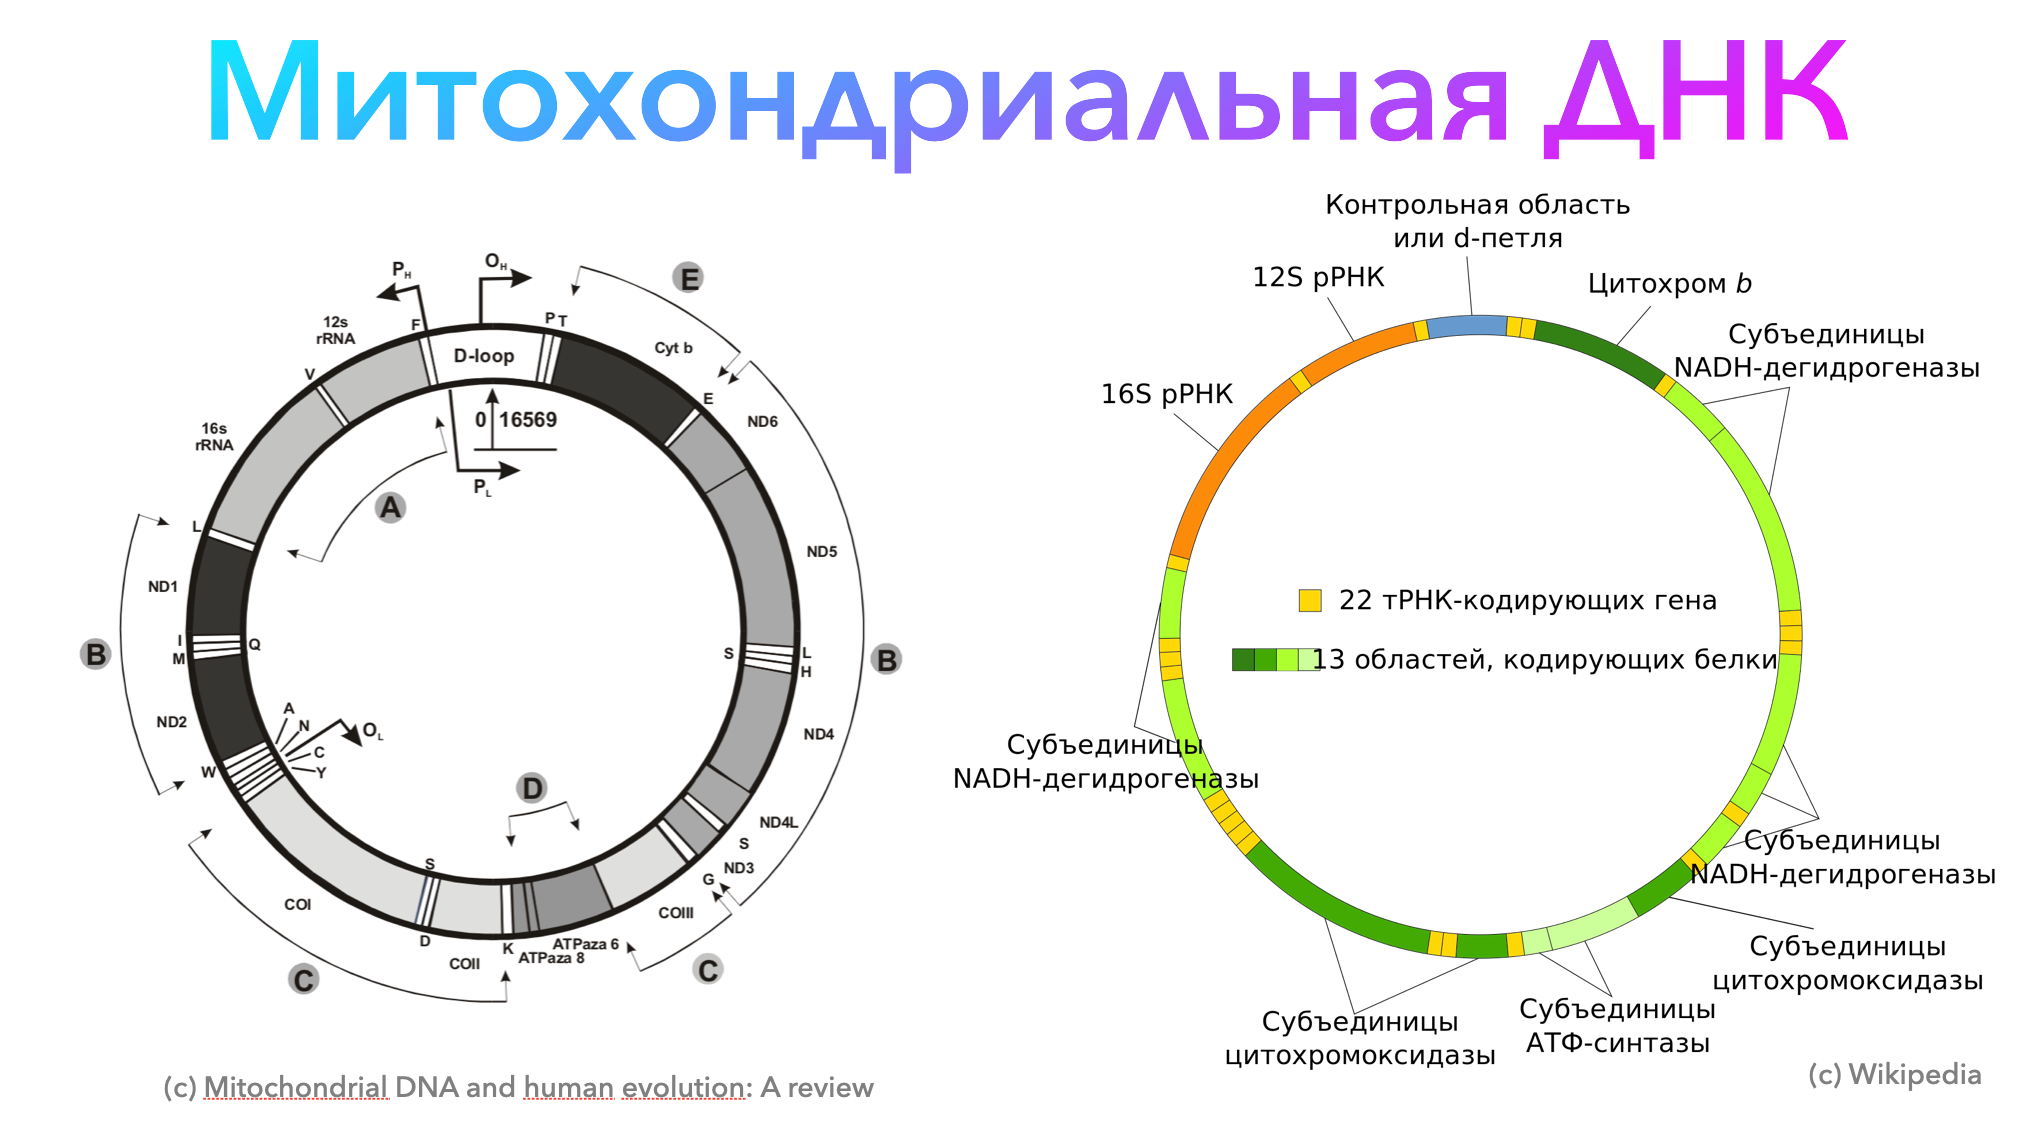
\includegraphics[width=\linewidth]{12_1}
	\caption{На рисунке изображен схематичное строение митохондриальной ДНК, которая включает в себя примерно 16,5 тысяч нуклеотидов и кодирует 13 полипептидов (зеленые области B, C, E, D); 2 рРНК (оранжевые области A); 22 тРНК (желтые области и белые на левом рисунке кроме d-петли) обеспечивающих трансляцию белков внутри митохондрии. D-loop это область не кодирующая часть содержащая два гипервариабельных участка (HVR1 HVR2)}
\end{figure}

\begin{figure}[H]
	\centering
	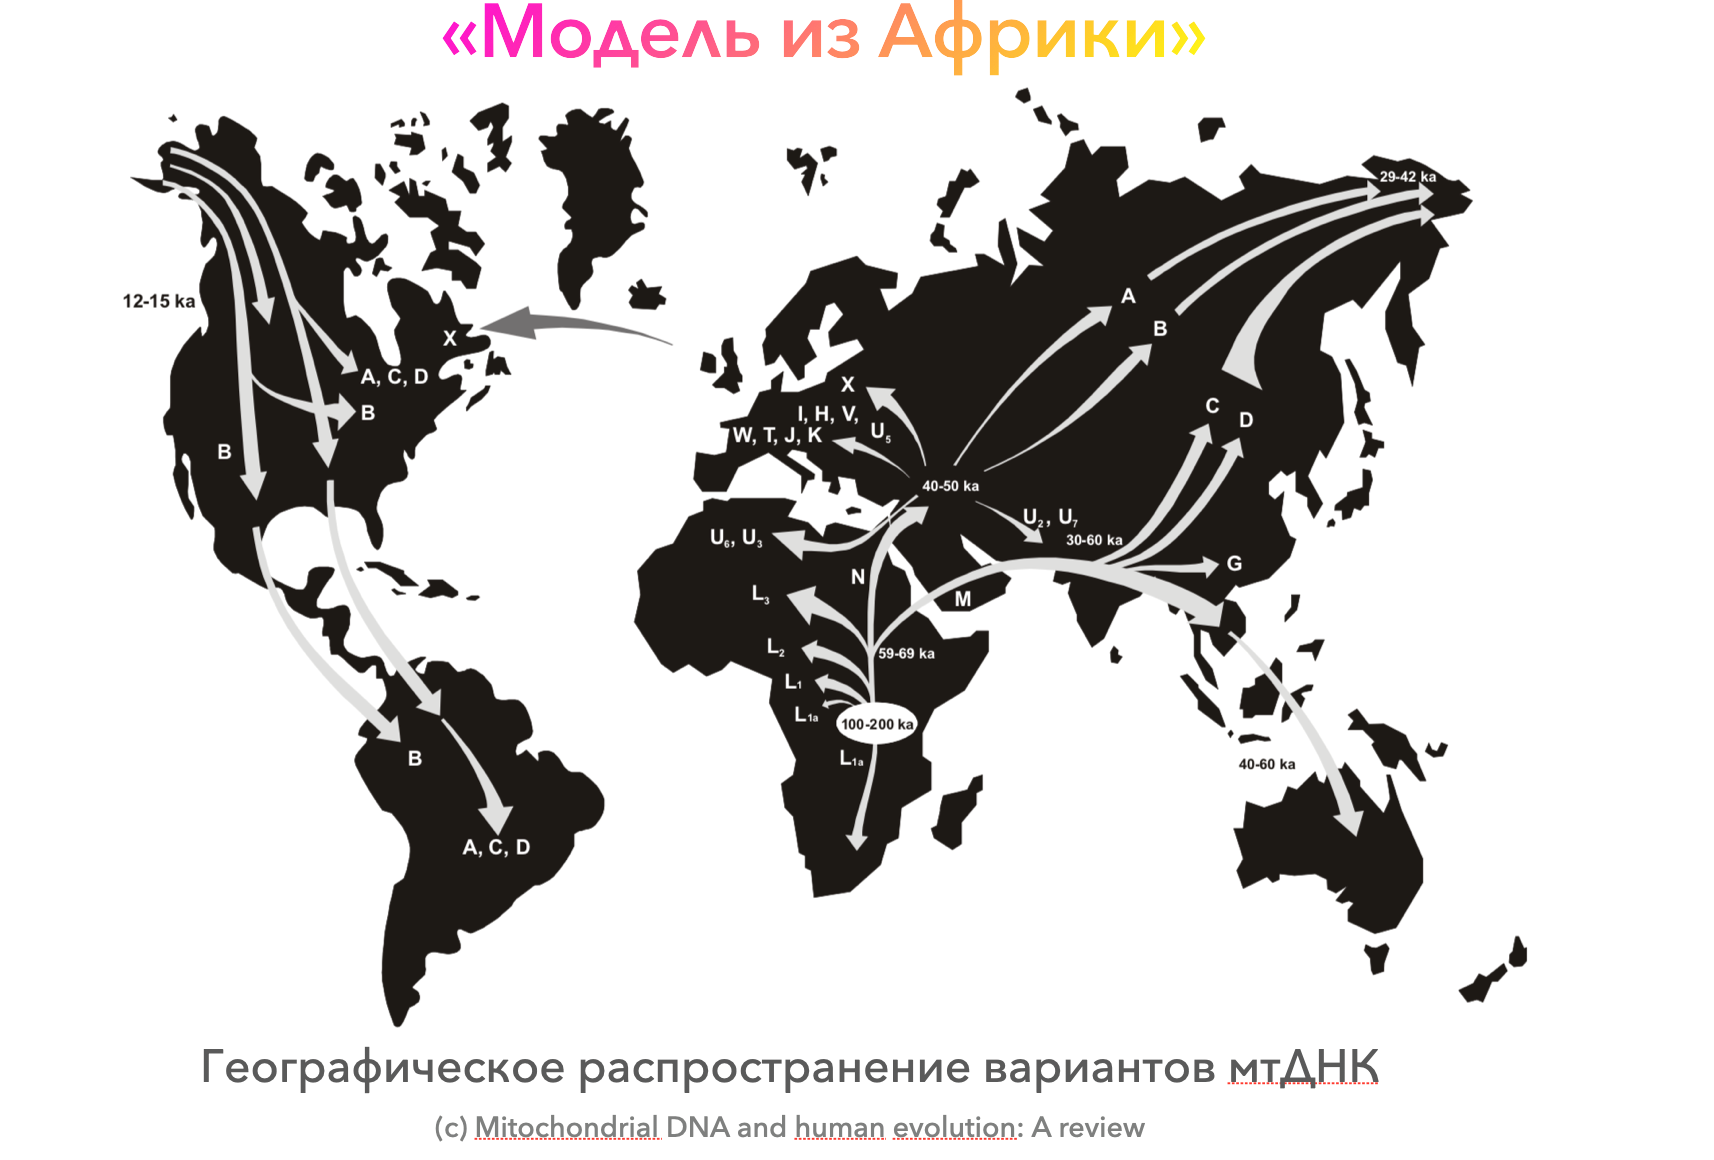
\includegraphics[width=\linewidth]{12_2}
	\caption{Одна из двух моделей расселения людей: «Модель из Африки». На рисунке изображено географическое распространение людей в ходе эволюции. Белая область на карте это место появления первой мтДНК (100-200 тысяч лет назад (ka)). Стрелки показывают распространение гаплогруппы (заглавные группы). Отслеживание миграций Homo sapiens с помощью мтДНК основано на наблюдении за тем, что появление определенных гаплотипов часто связано с определенными регионами мира, и на предположении, что это результат накопления различных мутаций.}
\end{figure}

\subsubsection{Для общего развития}

\begin{figure}[H]
	\centering
	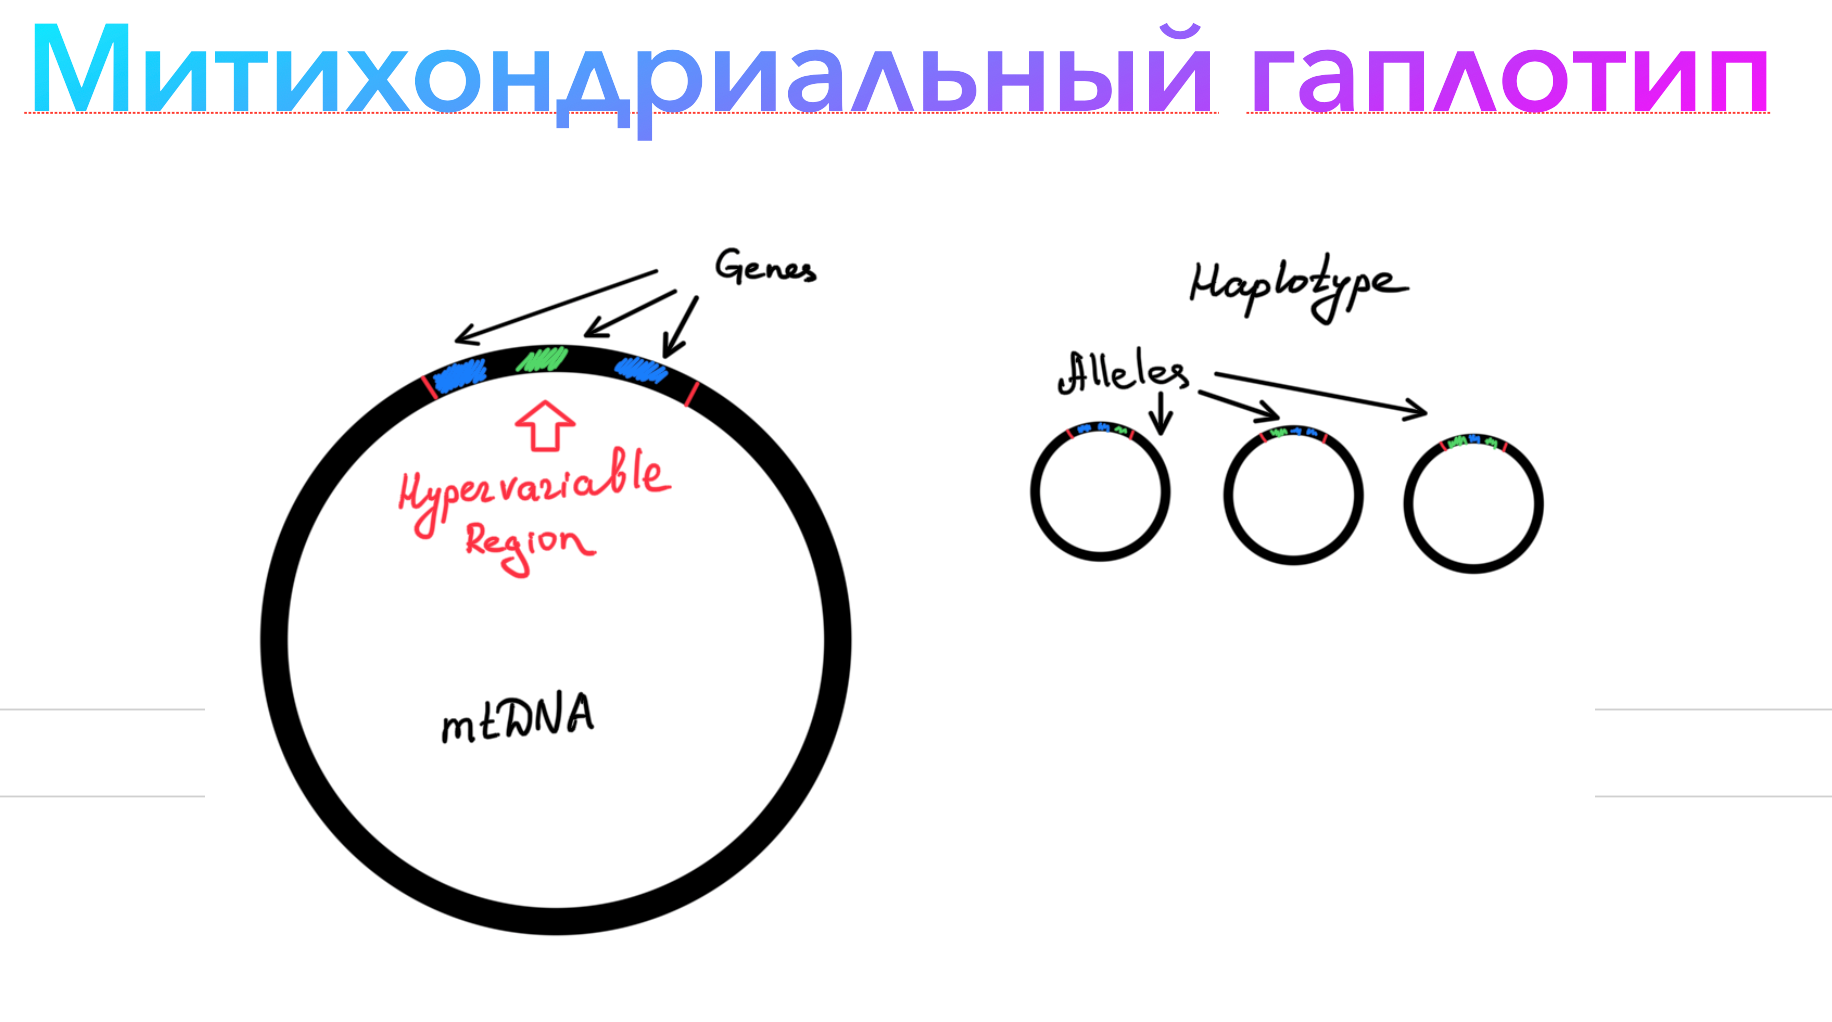
\includegraphics[width=\linewidth]{12_3}
\end{figure}

\begin{figure}[H]
	\centering
	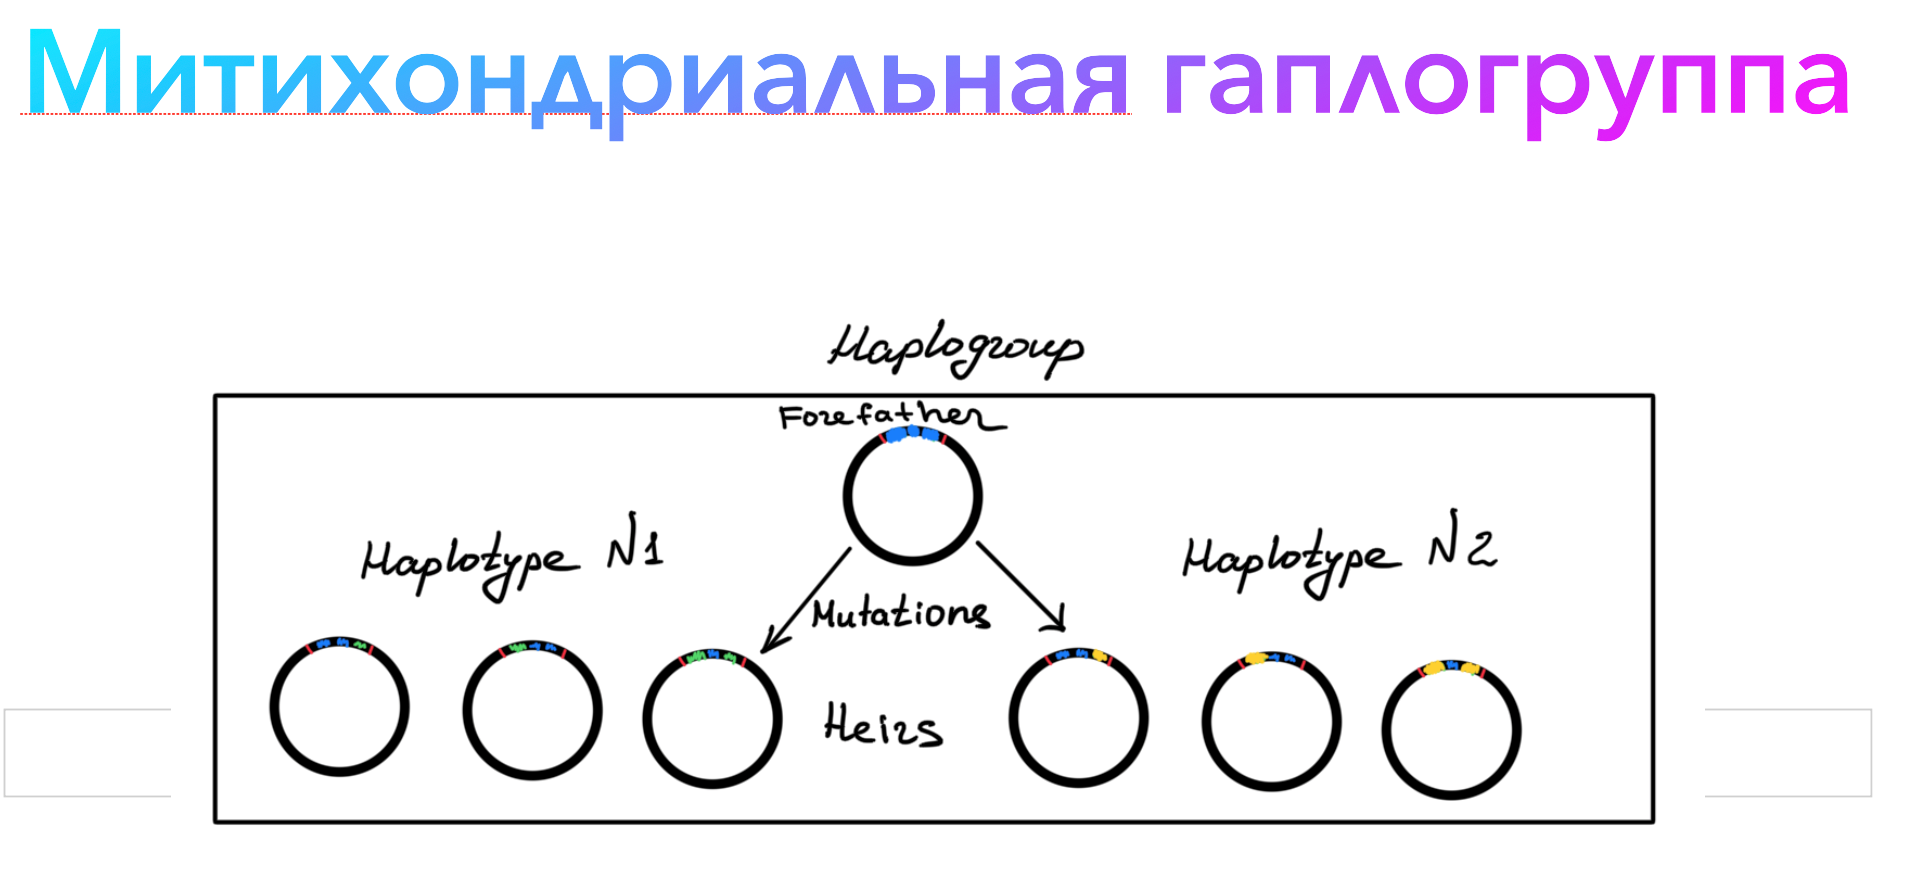
\includegraphics[width=\linewidth]{12_4}
\end{figure}